\chapter{Methods}\label{chapter:methods}

\section{Generalized Prony Method}

This section very closely follows the excellent phd thesis of Thomas Peter \cite{gen_prony_2013}.
It is assumed that every eigenspace $V_j$ of the linear operator $\hat{A}$ is one-dimensional. 
If the eigenspace is not one-dimensional, we choose a representative.
Thus for each eigenvalue $\lambda_j$ there exists a unique eigenvector $v_j$.

Furthermore, we assume that the function $f$ is $M$-sparse. Therefore, $M$ eigenfunctions suffice to represent the function exactly:
\begin{equation*}
    f = \sum_{j \in J} c_j\, v_j \qquad |J| = M
\end{equation*}
where $J$ is a proper subset of the set of all eigenfunctions of the linear operator $\hat{A}$.

Due to the linearity of the operator $\hat{A}$ it holds:
\begin{equation*}
    \hat{A}^k f = \sum_{j \in J} c_j\, \lambda_j^{k}\, v_j
\end{equation*}

Now we assume a linear functional $F$, such that $F v_j \neq 0$ holds for all $j \in I$. 
Then we can reconstruct $f$ with $2M$ values:
\begin{equation*}
    F(\hat{A}^k f), \qquad k = 0, \dots, 2M-1.
\end{equation*}

To find this reconstruction, we start with the general definition of a polynomial whose roots are given by $\lambda_j$:
\begin{equation*}
    P(z) := \prod_{j \in J} (z - \lambda_j)
\end{equation*}
Alternatively, this polynomial can be represented as a sum of trivial polynomials:
\begin{equation*}
    P(z) = \sum_{k=0}^{M} p_k\, z^{k}
\end{equation*}
where the $p_k$ are unknown and $p_M = 1$ is chosen. For $m \in \mathbb{N}$ we find:
\begin{align*}
    \sum_{k=0}^{M} p_k\, F(\hat{A}^{k+m} f) &= \sum_{k=0}^{M} p_k\, F\left( \sum_{j \in J} c_j\, \lambda_j^{k+m}\, v_j \right) = \\
    &= \sum_{j \in J} c_j\, \lambda_j^{m} \underbrace{\left( \sum_{k=0}^{M} p_k\, \lambda_j^{k} \right)}_{P(\lambda_j) = 0}\, F v_j = 0
\end{align*}

which yields with $p_M = 1$ the following linear system of equations for $p_k$:
\begin{equation*}
    \sum_{k=0}^{M-1} p_k\, F(\hat{A}^{k+m} f) = -F(\hat{A}^{M+m} f)
\end{equation*}

The matrix $\underline{H} = \left[ F(\hat{A}^{k+m} f) \right]_{k,m}$ is invertible.

\textbf{Proof:}
\begin{align*}
    \underline{H} = \left[ F(\hat{A}^{k+m} f) \right]_{k,m} &= \left[ \sum_{j \in J} c_j\, \lambda_j^{k+m}\, F(v_j) \right]_{k,m} \\
    &= \left[ \sum_{j \in J} \lambda_j^{k}\, c_j\, F(v_j)\, \lambda_j^{m} \right]_{k,m} \\
    &= \begin{pmatrix} \lambda_1^0 & \cdots & \lambda_M^0 \\ \lambda_1^1 & \cdots & \lambda_M^1 \\ \vdots & & \vdots \\ \lambda_1^{M-1} & \cdots & \lambda_M^{M-1} \end{pmatrix}
    \begin{pmatrix} c_1 F(v_1) & & \text{\Large 0} \\ & \ddots & \\ \text{\Large 0} & & c_M F(v_M) \end{pmatrix}
    \begin{pmatrix} \lambda_1^0 & \cdots & \lambda_1^{M-1} \\ \vdots & & \vdots \\ \lambda_M^0 & \cdots & \lambda_M^{M-1} \end{pmatrix}
\end{align*}

By assumption, none of the $c_j$ or $F(v_j)$ vanish, so the diagonal matrix is invertible. To show that the Vandermonde matrix
\begin{equation*}
    \underline{V}_{\lambda} := \left( \lambda_j^{k} \right)_{k=0,\, j \in J}^{M-1}
\end{equation*}
is also invertible, we use that for a square matrix invertibility is equivalent to linear independence of the rows and columns; We show it for the rows:
\begin{equation*}
    \sum_{k=0}^{M-1} c_k\, \lambda_j^{k} = 0 \qquad \forall j \in J \quad \text{with } |J| = M
\end{equation*}
A polynomial of degree $(M-1)$ has at most $(M-1)$ roots $\Rightarrow$ the system of equations cannot be satisfied $\Rightarrow$ all row vectors are linearly independent $\Rightarrow$ the matrix is invertible.

The $p_k$ are thus uniquely determined. Now we can find the eigenvalues $\lambda_j$ as roots of the polynomial:
\begin{equation*}
    P(z) = \sum_{k=0}^{M} p_k\, z^{k} \qquad \text{with } p_M = 1
\end{equation*}
and ,for example, using a power method, we can find the eigenfunctions $v_j$.

Alternatively, one can solve the system of equations $(\hat{A} - \lambda_j) v_j = 0$ directly or minimize $v_j^{\dagger}(\hat{A} - \lambda_j)^{\dagger}(\hat{A} - \lambda_j) v_j$.

Finally, we only need to solve
\begin{equation*}
    \left[ F(\hat{A}^k f) \right]_k = \left[ \lambda_j^{k} \right]_{k,\, j \in J}\, \left[ F(v_j) \right]_{j \in J}\, \left( c_j \right)_{j \in J}
\end{equation*}
for the vector $\left[ F(v_j) c_j \right]_{j \in J}$ with $k = 0, \dots, 2M-1$. So an overdetermined system of equations. Further,
if we know $\left[F(v_j)\right]_{j \in J}$ we can find the coefficients $\left[ c_j \right]_{j \in J}$.

\subsection{Derivation of the Prony Method from the generalized Prony Method}

The Prony method is obtained as a special case of the generalized Prony method by choosing $\hat{A} = \hat{T}(a) = \hat{T}_a$ and $F(f) = \int dx_0\, \delta(x_0)\, f(x_0)$. Here
\begin{equation*}
    \hat{T}(a)\, f(x_0) = f(x_0 + a).
\end{equation*}
With these definitions for the functional and the operator, we find the following formula for the coefficients of the characteristic polynomial:
\begin{align*}
    \sum_{k=0}^{M} p_k\, F(\hat{A}^{k+m} f) &= 0 \\
    \sum_{k=0}^{M} p_k \int dx_0\, \delta(x_0)\, \hat{T}_a^{k+m}\, f(x_0) &= 0 \\
    \sum_{k=0}^{M} p_k\, f((k+m)a) &= 0 \qquad 
\end{align*}

As a next step, we determine the roots of the characteristic polynomial / the eigenvalues of $\hat{T}_a$. In the case of the Prony method, we represent these as
\begin{equation*}
    \lambda_j = \exp(aT_j)
\end{equation*}
and thus find the eigenfunctions
\begin{equation*}
    \hat{T}_a\, \psi(x) = \exp(aT_j)\, \psi(x) \quad \Rightarrow \quad \psi(x) = \exp(T_j x).
\end{equation*}
To find the coefficients of the eigenfunction in the representation of $f(x)$, we only need to solve
\begin{equation*}
    F(\hat{A}^k f) = \sum_{j \in J} c_j\, \lambda_j^{k}\, F(v_j)
\end{equation*}
where
\begin{equation*}
    F(v_j) = \int dx_0\, \delta(x_0)\, \exp(T_j x_0) = 1
\end{equation*}

and
\begin{equation*}
    F(\hat{A}^k f) = F(\hat{T}_a^k f) = \int dx_0\, \delta(x_0)\, \hat{T}_a^k\, f(x_0) = f((k+1)a)
\end{equation*}
\begin{equation*}
    f(k) = \sum_{j \in J} c_j\, \lambda_j^{k} \qquad k = 0, \dots, 2M-1
\end{equation*}

The Prony method solves the uniquely determined system of equations with $k = 0, \dots, M-1$ ($1, \dots, M$) and not the overdetermined one, as is the case with the generalized Prony method.

\subsection{The Esprit Method}

The standard Prony Method can only utilize $2M-1$ function evaluations, where $M$ has to be known.
Therefore, we introduce the Esprit method, which can incorporate more data and allows us to formulate an educated 
guess about the sparsity $M$.
The idea is to replace the calculations of the $p_i$'s and instead directly calculate the zeros $\lambda_j$ of the polynomial:
\begin{equation*}
    \sum_k p_k z^k \qquad \text{with } \sum_k p_k \lambda_j^k = 0
\end{equation*}

As in the case of the Prony Method, we have:
\begin{equation*}
    \sum_k p_k\, F(\hat{A}^{k+m} f(x)) = 0
\end{equation*}
Let $(\underline{H})_{mk} = F(\hat{A}^{k+m} f(x)) = h(k+m)$, then
\begin{equation*}
    \underline{H}\, \vec{p} = 0
\end{equation*}
and with $p_{M'} = 1$
\begin{equation*}
    \begin{pmatrix} h(0) & \cdots & h(M'-1) \\ \vdots & & \vdots \\ h(M'-1) & \cdots & h(2M'-2) \end{pmatrix}
    \begin{pmatrix} p_0 \\ \vdots \\ p_{M'-1} \end{pmatrix}
    = \begin{pmatrix} -h(M') \\ \vdots \\ -h(2M'-1) \end{pmatrix}
\end{equation*}

Here we use $M'$, since $M'$ is an upper bound of the actual unknown sparsity $M$, so that we can use more data (in the case, where we know $M$).
Here we see that the companion matrix to the polynomial $C_P$ connects the following two matrices:
\begin{equation*}
    \underbrace{\begin{pmatrix} h(0) & \cdots & h(M'-1) \\ \vdots & & \vdots \\ h(M'-1) & \cdots & h(2M'-2) \end{pmatrix}}_{:= \underline{H}(0)}
    \underbrace{\begin{pmatrix} 0 & \cdots & & -p_0 \\ 1 & 0 & \cdots & -p_1 \\ & \ddots & \ddots & \vdots \\ 0 & & 1 & -p_{M'-1} \end{pmatrix}}_{\substack{\text{the minus does not} \\ \text{affect the zeros}}}
    = \underbrace{\begin{pmatrix} h(1) & \cdots & h(M') \\ \vdots & & \vdots \\ h(M') & \cdots & h(2M'-1) \end{pmatrix}}_{:= \underline{H}(1)}
\end{equation*}
and the eigenvalues and eigenvectors of the companion matrix are also the eigenvalues and eigenvectors of the generalized eigenvalue problem:
\begin{equation*}
    \left[ -\lambda_j\, \underline{H}(0) + \underline{H}(1) \right] \vec{v}_j = 0 \quad \Rightarrow \quad \left[ -\lambda_j\, \underline{H}(0) + \underline{H}(0)\, \underline{C}_P \right] \vec{v}_j = 0
\end{equation*}
since $\underline{C}_P\vec{v}_j = \lambda_j \vec{v}_j$.

Solving the full generalized eigenproblem will, in general, give too many eigenvalues. Therefore, it is necessary to isolate the dominating components of the large matrix. This can be achieved efficiently using the singular value decomposition:

Let $\underline{H}$ denote the matrix, which contains all columns of $\underline{H}(0)$ and $\underline{H}(1)$ respectively:
\begin{equation*}
    \underline{H} = \begin{pmatrix} h(0) & \cdots & h(M') \\ \vdots & & \vdots \\ h(M'-1) & \cdots & h(2M'-1) \end{pmatrix} = \underline{U}\,\underline{S}\,\underline{V}
\end{equation*}
and let again $\underline{V}(0)$ denote the first $M'$ columns of $\underline{V}$ and $\underline{V}(1)$ the last $M'$ columns of $\underline{V}$. Then we find:
\begin{equation*}
    \underline{H}(0) = \underline{U}\,\underline{S}\,\underline{V}(0) \qquad\qquad \underline{H}(1) = \underline{U}\,\underline{S}\,\underline{V}(1)
\end{equation*}

Assuming the sparsity $M$ is known, the $M$ rows of $\underline{V}$ and the $M$ columns of $\underline{U}$ corresponding to the largest singular values are retained. The magnitude of the discarded singular values provide a measure of quality of the fit and the noise level present in the data.

If $M$ is unknown, we can obtain a nice guess at this point,an initial estimate can be obtained by examining the singular value spectrum, for example by identifying a significant drop in the singular values or by using cutoff values.

The generalized eigenproblem can be simplified using the SVD expressions:
\begin{equation*}
    -\lambda_j\, \underline{H}(0) + \underline{H}(1) = -\lambda_j\, \underline{U}\,\underline{S}\,\underline{V}(0) + \underline{U}\,\underline{S}\,\underline{V}(1)
\end{equation*}
or
\begin{equation*}
    = -\lambda_j\, \underline{U}'\,\underline{S}'\,\underline{V}'(0) + \underline{U}'\,\underline{S}'\,\underline{V}'(1)
\end{equation*}

where the primes denote the reduced matrices.

\begin{equation*}
    \left( -\lambda_j\, \underline{U}'\,\underline{S}'\,\underline{V}'(0) + \underline{U}'\,\underline{S}'\,\underline{V}'(1) \right) \vec{v}_j = \vec{0}
\end{equation*}
\begin{equation*}
    \left( -\lambda_j\, \underline{V}'(0) + \underline{V}'(1) \right) \vec{v}_j = \vec{0}
\end{equation*}
\begin{equation*}
    \underline{V}'(0)^{-1}\, \underline{V}'(1)\, \vec{v}_j = \lambda_j\, \vec{v}_j
\end{equation*}
or formulated differently, we want to solve the eigenproblem:
\begin{equation*}
    \underline{A}\, \vec{v}_j = \lambda_j\, \vec{v}_j
\end{equation*}
where $\underline{A}$ solves:
\begin{equation*}
    \underline{V}'(0)\, \underline{A} = \underline{V}'(1)
\end{equation*}
This will give us the eigenvalues and from these we proceed as usual.




\section{DMRG}

\subsection{Matrix Implementation}

\subsubsection{Partial trace --- motivation}

Assume a large system is composed of two subsystems $A$ and $B$, whose
Hilbert spaces have dimensionality $n_A$ and $n_B$ respectively. Further, let
$O\in\mathbb C^{n_A\times n_A}$ be an observable of subsystem $A$. Then
the reduced density matrix

\begin{equation}
\rho_A = \operatorname{Tr}_B[\rho]
\end{equation}

is the appropriate representation of the state $\rho$ on subsystem $A$
in the following sense:

\begin{equation}
\mathbb E\big[O\otimes I\big] = \operatorname{Tr}\big[(O\otimes I)\,\rho\big]
= \operatorname{Tr}_A\big[O\,\operatorname{Tr}_B[\rho]\big] = \operatorname{Tr}_A\big[O\rho_A\big] = \mathbb E_A[O]
\end{equation}

\paragraph{Proof.} Define $\bar O = O\otimes I$, meaning

\begin{equation}
\bar O_{ii',\,jj'} = \begin{cases} O_{ij} & \text{if } i'=j'\\[2pt] 0 & \text{if } i'\neq j'\end{cases}
\end{equation}

with $i,j\in[0,n_A)$ and $i',j'\in[0,n_B)$.

\begin{align}
\operatorname{Tr}\big[\bar O\rho\big]
&= \sum_{i,j,i',j'}\bar O_{ii',\,jj'}\;\rho_{jj',\,ii'}
= \sum_{i,j}O_{ij}\sum_{i'}\rho_{ji',\,ii'}\\
&= \sum_{i,j}O_{ij}\,\operatorname{Tr}_B[\rho]_{j,i}
= \operatorname{Tr}_A\big[O\rho_A\big]
\end{align}

\paragraph{Proving uniqueness.}
We are going to show that two matrices $\rho_A$ and $\rho_A'$, which
both satisfy

\begin{equation}
\operatorname{Tr}_A\big[O\rho_A\big] = \operatorname{Tr}\big[(O\otimes I)\rho\big] = \operatorname{Tr}\big[O\rho_A'\big],
\end{equation}

agree entry for entry. Linearity of matrix multiplication and trace
give:

\begin{equation}
\operatorname{Tr}_A\big[O(\rho_A-\rho_A')\big] = \operatorname{Tr}_A\big[O\rho_A\big] - \operatorname{Tr}_A\big[O\rho_A'\big] = 0.
\end{equation}

This must hold for all $O\in\mathbb C^{n_A\times n_A}$. We choose

\begin{equation}
O^{(\alpha,\beta)}_{ij} = \begin{cases}1 & \text{if } i=\alpha \text{ and } j=\beta\\ 0 & \text{else}\end{cases}
\end{equation}

so matrices with only a single non-zero entry. Then we find $\forall \alpha ,\beta \in [0,n_{A})$:

\begin{align}
0 &= \operatorname{Tr}_A\big[O^{(\alpha,\beta)}(\rho_A-\rho_A')\big] = \sum_{i,j}O^{(\alpha,\beta)}_{ij}\,(\rho_A-\rho_A')_{ji}\\
0 &= (\rho_A-\rho_A')_{\beta,\alpha}\\
(\rho_A')_{\beta,\alpha} &= (\rho_A)_{\beta,\alpha} \qquad\qquad\square
\end{align}

\subsubsection{Infinite DMRG -- Background}

Used to estimate the energy density of the groundstate $\dfrac{E}{L}$. 
Where $L$ denotes the number of sites.

All terms of the Hamiltonian for which the $i$-th site is the leftmost
site on which the operator acts are therefore

\begin{align}
H^{(i)} &= \sum_{n=1}^{N}\hat O^{(n)}_{i,\dots,i+n-1}\notag\\
&= \sum_{n=1}^{N}\big[O^{(n)}\big]_{\sigma_i,\dots,\sigma_{i+n-1};\,\sigma_i',\dots,\sigma_{i+n-1}'}\;
\big|\sigma_i\cdots\sigma_{i+n-1}\big\rangle\big\langle\sigma_i'\cdots\sigma_{i+n-1}'\big|,
\end{align}

Summation over all the sigmas is implied.

\subsubsection{Algorithm -- exhaustive}

The following describes a single iteration, which is repeated until
convergence.

We start with the ``left'' and ``right'' bases

\begin{equation}
\big\{\,|\alpha\rangle \;\big|\; \alpha\in[0,\chi)\,\big\}
\qquad\text{and}\qquad
\big\{\,|\beta\rangle \;\big|\; \beta\in[0,\chi)\,\big\},
\end{equation}

where $\chi$ is usually bounded from above by $\chi_{\max}$, which can
be chosen. The bases were either determined in the previous iteration,
or they span a one-dimensional space, i.e.\ $\alpha$ and $\beta$ are
dummy indices.

Now we expand the space within which we can search for the ground
state, from

\begin{equation}
\operatorname{span}\Big(\big\{\,|\alpha,\beta\rangle \;\big|\; \alpha,\beta\in[0,\chi)\,\big\}\Big)
\end{equation}

to

\begin{equation}
\operatorname{span}\Big(\big\{\,|\alpha,\sigma_L,\sigma_R,\beta\rangle \;\big|\; \alpha,\beta\in[0,\chi),\ \sigma_L,\sigma_R\in[0,d)\,\big\}\Big),
\end{equation}

where $d$ is the dimension of the local space of a single physical leg,
i.e.\ $d=2$ for spinless fermions and $d=4$ for spinful fermions.

We assume that all operators act on this space, or can be extended to
operators acting on that space by taking a Kronecker product with an
identity matrix of the appropriate dimension. We will see later how to
bring the operators into the correct form.

Now we compute the ground state of the Hamiltonian

\begin{equation}
H = \sum_{\substack{\alpha,\sigma_L,\sigma_R,\beta\\ \alpha',\sigma_L',\sigma_R',\beta'}}
H_{\alpha\sigma_L\sigma_R\beta,\;\alpha'\sigma_L'\sigma_R'\beta'}\;
\big|\alpha\sigma_L\sigma_R\beta\big\rangle\big\langle\alpha'\sigma_L'\sigma_R'\beta'\big|.
\end{equation}

and denote the ground state by

\begin{equation}
|\Psi\rangle = \sum_{\alpha,\sigma_L,\sigma_R,\beta}
\Psi_{\alpha\sigma_L\sigma_R\beta}\;\big|\alpha\,\sigma_L\,\sigma_R\,\beta\big\rangle.
\end{equation}

From the state we construct the density matrix:

\begin{equation}
\rho = |\Psi\rangle\langle\Psi| = \sum_{\substack{\alpha,\sigma_L,\sigma_R,\beta\\ \alpha',\sigma_L',\sigma_R',\beta'}}
\Psi_{\alpha\sigma_L\sigma_R\beta}\,\Psi^*_{\alpha'\sigma_L'\sigma_R'\beta'}\;
\big|\alpha\sigma_L\sigma_R\beta\big\rangle\big\langle\alpha'\sigma_L'\sigma_R'\beta'\big|.
\end{equation}

Now we want to reduce the amount of information we have to store,
i.e.\ we want to reduce the dimension of the left and right subspace from $d\cdot\chi$ to
dimension $\chi$.

\paragraph{Step: $|\alpha\,\sigma_L\rangle \to |\alpha^{\mathrm{new}}\rangle$.}
Trace out the right half:

\begin{align}
\rho_L = \operatorname{tr}_R[\rho]
&= \sum_{\substack{\alpha,\sigma_L,\sigma_R,\beta\\ \alpha',\sigma_L'}}
\Psi_{\alpha\sigma_L\sigma_R\beta}\,\Psi^*_{\alpha'\sigma_L'\sigma_R\beta}\;
\big|\alpha\sigma_L\big\rangle\big\langle\alpha'\sigma_L'\big|\\
&= \sum_{\alpha,\sigma_L,\,\alpha',\sigma_L'}
\big(\underline{\Psi}\underline{\Psi}^\dagger\big)_{\alpha\sigma_L,\,\alpha'\sigma_L'}\;
\big|\alpha\sigma_L\big\rangle\big\langle\alpha'\sigma_L'\big|,
\end{align}

where $(\underline{\Psi})_{i,j} = \Psi_{ij}$ (just reshaped into a matrix).

Now we only want to keep the $\chi$ components that hold the most
``information'' about the state.

This corresponds to finding the eigenvectors with the largest
magnitude eigenvalues of the matrix $\underline{M} = \underline{\Psi}\,\underline{\Psi}^\dagger$.
(Note: $\underline{M}$ is positive semi-definite hermitian Matrix, so largest magnitude
eqauls largest algebraically)
However, we can skip the calculation of $\underline{M}$ and directly
compute a singular value decomposition of
$\underline{\Psi} = \underline{U}\,\underline{S}\,\underline{V}^\dagger$:

\begin{equation}
\underline{M} = \underline{\Psi}\,\underline{\Psi}^\dagger
= \underline{U}\,\underline{S}\,\underline{S}^*\,\underline{U}^\dagger
= \underline{U}\,\underline{S}^2\,\underline{U}^\dagger.
\end{equation}

Where $\underline{S}^*=\underline{S}$, since singular values are real (and positive or zero).
So we find that the columns of $\underline{U}$ are the eigenvectors of
$\underline{M}$, and the corresponding eigenvalues are the singular
values squared.

Now we find the reduced representation of $\underline{M}$ by
neglecting the eigenvectors/columns of $\underline{U}$ that correspond
to the smallest singular values.

We can reinsert the reduced representation into the formula for
$\rho_L$:

\begin{align}
\rho_L &= \sum_{\alpha,\sigma_L,\,\alpha',\sigma_L'}
\big(\underline{M}^{(\mathrm{red})}\big)_{\alpha\sigma_L,\,\alpha'\sigma_L'}\;
\big|\alpha\sigma_L\big\rangle\big\langle\alpha'\sigma_L'\big|\\
&= \sum_{\substack{\alpha,\sigma_L,\,\alpha',\sigma_L'\\ \alpha_{\mathrm{new}},\,\alpha_{\mathrm{new}}'}}
\big(\underline{U}^{(\mathrm{red})}\big)_{\alpha\sigma_L,\,\alpha_{\mathrm{new}}}
\big(\underline{S}^{(\mathrm{red})}\big)^2_{\alpha_{\mathrm{new}},\,\alpha_{\mathrm{new}}}
\big(\underline{U}^{(\mathrm{red})\dagger}\big)_{\alpha_{\mathrm{new}},\,\alpha'\sigma_L'}\;
\big|\alpha\sigma_L\big\rangle\big\langle\alpha'\sigma_L'\big| \\
&= \sum_{\alpha_{\mathrm{new}}} \underline{S}^{(\mathrm{red})}\big)^2_{\alpha_{\mathrm{new}},\,\alpha_{\mathrm{new}}} \big|\alpha_{\mathrm{new}}\big\rangle\big\langle\alpha_{\mathrm{new}}\big|
\end{align}

with

\begin{equation}
\boxed{\;|\alpha_{\mathrm{new}}\rangle = \sum_{\alpha,\sigma_L}\big(\underline{U}^{(\mathrm{red})}\big)_{\alpha\sigma_L,\,\alpha_{\mathrm{new}}}\;|\alpha\sigma_L\rangle\;}
\end{equation}

and 

\begin{equation}
\boxed{\;\langle\alpha_{\mathrm{new}}| = \sum_{\alpha,\sigma_L}\big(\underline{U}^{(\mathrm{red})\dagger}\big)_{\alpha_{\mathrm{new}},\alpha\sigma_L}\;\langle\alpha\sigma_L|\;}
\end{equation}

We can also find the typical matrix-vector-notation relationship by
``moving'' the matrix from the basis elements onto the coefficients:

\begin{align}
|v\rangle &= \sum_{\alpha_{\mathrm{new}}}\big(\vec v_{\mathrm{new}}\big)_{\alpha_{\mathrm{new}}}\;|\alpha_{\mathrm{new}}\rangle\\
&= \sum_{\alpha_{\mathrm{new}}}\big(\vec v_{\mathrm{new}}\big)_{\alpha_{\mathrm{new}}}
\sum_{\alpha,\sigma_L}\big(\underline{U}^{(\mathrm{red})}\big)_{\alpha\sigma_L,\,\alpha_{\mathrm{new}}}\;|\alpha\sigma_L\rangle\\
&= \sum_{\alpha,\sigma_L}\Big(\underline{U}^{(\mathrm{red})}\,\vec v_{\mathrm{new}}\Big)_{\alpha\sigma_L}\;|\alpha\sigma_L\rangle
\end{align}

or in matrix-vector notation, where we do not explicitly denote the
basis:

\begin{equation}
\boxed{\;\vec v_{\mathrm{old}} = \underline{U}^{(\mathrm{red})}\,\vec v_{\mathrm{new}}\;}
\end{equation}

We can also find the inverse relationship:

\begin{align}
|v\rangle &= \sum_{\alpha_{\mathrm{new}}}\big(\vec v_{\mathrm{new}}\big)_{\alpha_{\mathrm{new}}}\;|\alpha_{\mathrm{new}}\rangle\\
&= \sum_{\alpha_{\mathrm{new}}}\big(\vec v_{\mathrm{new}}\big)_{\alpha_{\mathrm{new}}}
\sum_{\alpha,\sigma_L}\big(\underline{U}^{(\mathrm{red})}\big)_{\alpha\sigma_L,\,\alpha_{\mathrm{new}}}\;|\alpha\sigma_L\rangle\\
|v\rangle &\overset{!}{=} \sum_{\alpha_{\mathrm{new}}}\big(\vec v_{\mathrm{new}}\big)_{\alpha_{\mathrm{new}}}
\sum_{\alpha,\sigma_L}\big(\underline{U}^{(\mathrm{red})}\big)_{\alpha\sigma_L,\,\alpha_{\mathrm{new}}}
\sum_{\alpha'_{\mathrm{new}}}\big(\underline{M}\big)_{\alpha\sigma_L,\,\alpha'_{\mathrm{new}}}\;|\alpha'_{\mathrm{new}}\rangle
\end{align}

so we find

\begin{equation}
\sum_{\alpha,\sigma_L}\big(\underline{U}^{(\mathrm{red})}\big)_{\alpha\sigma_L,\,\alpha_{\mathrm{new}}}
\sum_{\alpha'_{\mathrm{new}}}\big(\underline{M}\big)_{\alpha\sigma_L,\,\alpha'_{\mathrm{new}}}\;|\alpha'_{\mathrm{new}}\rangle
\overset{!}{=} |\alpha_{\mathrm{new}}\rangle
\end{equation}

\begin{equation}
\sum_{\alpha'_{\mathrm{new}}}\big(\underline{M}^{T}\,\underline{U}^{(\mathrm{red})}\big)_{\alpha'_{\mathrm{new}},\,\alpha_{\mathrm{new}}}\;|\alpha'_{\mathrm{new}}\rangle
\overset{!}{=} |\alpha_{\mathrm{new}}\rangle
\end{equation}

We choose

\begin{equation}
\underline{M}^{T} = \underline{U}^{(\mathrm{red})\dagger}.
\end{equation}

since any $\underline{U}^{(\mathrm{red})\dagger} + \underline{K}$
where $\underline{K}\underline{U}^{(\mathrm{red})}=0$ would also fulfill
the requirement. Here one could choose for any row of $\underline{K}$ any linear combination
of the complex conjugates of the neglected eigenvectors.
Inserting back into the expansion of $|\alpha\sigma_L\rangle$:

\begin{equation}\label{eq:left-side-basis-el-ket}
\boxed{\;|\alpha\sigma_L\rangle = \sum_{\alpha_{\mathrm{new}}}\big(\underline{U}^{(\mathrm{red})\dagger}\big)_{\alpha_{\mathrm{new}},\,\alpha\sigma_L}\;|\alpha_{\mathrm{new}}\rangle\;}
\end{equation}

analogously we find

\begin{equation}\label{eq:left-side-basis-el-bra}
\boxed{\;\langle\alpha\sigma_L| = \sum_{\alpha_{\mathrm{new}}}\big(\underline{U}^{(\mathrm{red})}\big)_{\,\alpha\sigma_L,\alpha_{\mathrm{new}}}\;\langle\alpha_{\mathrm{new}}|\;}
\end{equation}

We can use the projective basis transformations \eqref{eq:left-side-basis-el-ket} and
\eqref{eq:left-side-basis-el-bra} to find the reduced representation of an operator
in the new basis:

\begin{equation}
\hat O^{(L)} = \sum_{\alpha\sigma_L,\,\alpha'\sigma_L'}
\big(\underline{O}^{(L)}\big)_{\alpha\sigma_L,\,\alpha'\sigma_L'}\;
\big|\alpha\sigma_L\big\rangle\big\langle\alpha'\sigma_L'\big|
\end{equation}

\begin{align}
\hat O^{(L)}_{\mathrm{red}} = \sum_{\alpha\sigma_L,\,\alpha'\sigma_L'}
\big(\underline{O}^{(L)}\big)_{\alpha\sigma_L,\,\alpha'\sigma_L'}
&\sum_{\alpha_{\mathrm{new}}}\big(\underline{U}^{(\mathrm{red})\dagger}\big)_{\alpha_{\mathrm{new}},\,\alpha\sigma_L}\;\big|\alpha_{\mathrm{new}}\big\rangle\notag\\
&\times\sum_{\alpha'_{\mathrm{new}}}\big(\underline{U}^{(\mathrm{red})}\big)_{\alpha'\sigma_L',\,\alpha'_{\mathrm{new}}}\;\big\langle\alpha'_{\mathrm{new}}\big|
\end{align}

\begin{equation}\label{eq:projective-basis-trafo-left}
\boxed{\;\hat O^{(L)}_{\mathrm{red}} = \sum_{\alpha_{\mathrm{new}},\,\alpha'_{\mathrm{new}}}
\Big(\underline{U}^{(\mathrm{red})\dagger}\,\underline{O}^{(L)}\,\underline{U}^{(\mathrm{red})}\Big)_{\alpha_{\mathrm{new}},\,\alpha'_{\mathrm{new}}}\;
\big|\alpha_{\mathrm{new}}\big\rangle\big\langle\alpha'_{\mathrm{new}}\big|\;}
\end{equation}

For this procedure to be applicable we obviously require $\hat O^{(L)}$
to act only on the left subspace, meaning that an operator that would
also act on the right subspace would have to be given in a
Kronecker-factorized form. However, if one wants to avoid computing the
Kronecker factorization, the formula can easily be extended to

\begin{equation}
\boxed{\;\hat O_{\mathrm{red}} = \sum_{\alpha_{\mathrm{new}},\,\alpha'_{\mathrm{new}},\,\gamma,\gamma'}
\Big(\big(\underline{U}^{(\mathrm{red})\dagger}\otimes \underline{I}\big)\,\underline{O}\,\big(\underline{U}^{(\mathrm{red})}\otimes \underline{I}\big)\Big)_{\alpha_{\mathrm{new}}\sigma,\;\alpha'_{\mathrm{new}}\sigma'}\;
\big|\alpha_{\mathrm{new}}\,\gamma\big\rangle\big\langle\alpha'_{\mathrm{new}}\,\gamma'\big|\;}
\end{equation}

Remains to change the right basis.

\begin{align}
\rho_R = \operatorname{tr}_L[\rho]
&= \operatorname{tr}_L\Big[\sum_{\substack{\alpha\sigma_L\sigma_R\beta\\ \alpha'\sigma_L'\sigma_R'\beta'}}
\Psi_{\alpha\sigma_L\sigma_R\beta}\,\Psi^*_{\alpha'\sigma_L'\sigma_R'\beta'}\;
\big|\alpha\sigma_L\sigma_R\beta\big\rangle\big\langle\alpha'\sigma_L'\sigma_R'\beta'\big|\Big]\\
&= \sum_{\substack{\sigma_R,\beta\\ \sigma_R',\beta'}}
\big(\underline{\Psi}^{T}\underline{\Psi}^{*}\big)_{\sigma_R\beta,\,\sigma_R'\beta'}\;
\big|\sigma_R\beta\big\rangle\big\langle\sigma_R'\beta'\big|\\
&= \sum_{\substack{\sigma_R,\beta\\ \sigma_R',\beta'}}\sum_{\beta_{\mathrm{new}},\beta'_{\mathrm{new}}}
\big(\underline{V}^{(\mathrm{red})*}\big)_{\sigma_R\beta,\,\beta_{\mathrm{new}}}
\big(\underline{S}^{(\mathrm{red})2}\big)_{\beta_{\mathrm{new}},\,\beta'_{\mathrm{new}}}
\big(\underline{V}^{(\mathrm{red})T}\big)_{\beta'_{\mathrm{new}},\,\sigma_R'\beta'}\;
\big|\sigma_R\beta\big\rangle\big\langle\sigma_R'\beta'\big|\\
&= \sum_{\beta_{\mathrm{new}},\,\beta'_{\mathrm{new}}}
\big|\beta_{\mathrm{new}}\big\rangle\,\big(\underline{S}^{(\mathrm{red})2}\big)_{\beta_{\mathrm{new}},\,\beta'_{\mathrm{new}}}\,\big\langle\beta'_{\mathrm{new}}\big|
\end{align}

So we can read off:

\begin{equation}
\boxed{\;\big|\beta_{\mathrm{new}}\big\rangle = \sum_{\sigma_R,\beta}\big(\underline{V}^{(\mathrm{red})}\big)^{*}_{\sigma_R\beta,\,\beta_{\mathrm{new}}}\;\big|\sigma_R\beta\big\rangle\;}
\end{equation}

and

\begin{equation}
\boxed{\;\big\langle\beta_{\mathrm{new}}\big| = \sum_{\sigma_R,\beta}\big(\underline{V}^{(\mathrm{red})}\big)^{T}_{\beta_{\mathrm{new}},\,\sigma_R\beta}\;\big\langle\sigma_R\beta\big|\;}
\end{equation}

and from

\begin{equation}
\big|\beta_{\mathrm{new}}\big\rangle = \sum_{\sigma_R,\beta}\big(\underline{V}^{(\mathrm{red})}\big)^{*}_{\sigma_R\beta,\,\beta_{\mathrm{new}}}\;\big|\sigma_R\beta\big\rangle
\end{equation}

we want to find

\begin{equation}
\big|\sigma_R\beta\big\rangle \approx \sum_{\beta'_{\mathrm{new}}}\big(\underline{M}\big)_{\sigma_R\beta,\,\beta'_{\mathrm{new}}}\;\big|\beta'_{\mathrm{new}}\big\rangle,
\end{equation}

the approximation of $|\sigma_R\beta\rangle$ within the space spanned by
$\big\{\,|\beta'_{\mathrm{new}}\rangle \;\big|\; \beta'_{\mathrm{new}}\in[0,\chi)\,\big\}$, such that

\begin{equation}
\big|\beta_{\mathrm{new}}\big\rangle = \sum_{\sigma_R,\beta}\big(\underline{V}^{(\mathrm{red})}\big)^{*}_{\sigma_R\beta,\,\beta_{\mathrm{new}}}
\sum_{\beta'_{\mathrm{new}}}\big(\underline{M}\big)_{\sigma_R\beta,\,\beta'_{\mathrm{new}}}\;\big|\beta'_{\mathrm{new}}\big\rangle.
\end{equation}

This implies

\begin{equation}
\underline{M}^{T}\,\big(\underline{V}^{(\mathrm{red})}\big)^{*} \overset{!}{=} \mathbb{1}
\end{equation}

and we choose

\begin{equation}
\underline{M} = \underline{V}^{(\mathrm{red})}.
\end{equation}

Important: $\big(\underline{V}^{(\mathrm{red})}\big)^{\dagger}$ has shape $(\chi,\;d\cdot\chi)$.

which gives

\begin{equation}
\boxed{\;\big|\sigma_R\beta\big\rangle = \sum_{\beta'_{\mathrm{new}}}\big(\underline{V}^{(\mathrm{red})}\big)^{T}_{\beta'_{\mathrm{new}},\,\sigma_R\beta}\;\big|\beta'_{\mathrm{new}}\big\rangle\;}
\end{equation}

Analogously we find:

\begin{equation}
\boxed{\;\big\langle\sigma_R\beta\big| = \sum_{\beta_{\mathrm{new}}}\big(\underline{V}^{(\mathrm{red})}\big)^{*}_{\sigma_R\beta,\,\beta_{\mathrm{new}}}\;\big\langle\beta_{\mathrm{new}}\big|\;}
\end{equation}

Now we can apply the projective basis transformation directly to an
operator:

\begin{equation}
\hat O^{(R)} = \sum_{\substack{\sigma_R\beta\\ \sigma_R'\beta'}}
\big(\underline{O}^{(R)}\big)_{\sigma_R\beta,\,\sigma_R'\beta'}\;
\big|\sigma_R\beta\big\rangle\big\langle\sigma_R'\beta'\big|
\end{equation}

\begin{equation}\label{eq:projective-basis-trafo-right}
\boxed{\;\hat O^{(R)}_{\mathrm{red}} = \sum_{\beta_{\mathrm{new}},\,\beta'_{\mathrm{new}}}
\Big(\big(\underline{V}^{(\mathrm{red})}\big)^{T}\,\underline{O}^{(R)}\,\big(\underline{V}^{(\mathrm{red})}\big)^{*}\Big)_{\beta_{\mathrm{new}},\,\beta'_{\mathrm{new}}}\;
\big|\beta_{\mathrm{new}}\big\rangle\big\langle\beta'_{\mathrm{new}}\big|\;}
\end{equation}

or in the expanded version

\begin{equation}
\boxed{\;\hat O_{\mathrm{red}} = \sum_{\substack{\beta_{\mathrm{new}},\,\beta'_{\mathrm{new}}\\ \gamma,\gamma'}}
\Big(\big(\underline{I}\otimes\big(\underline{V}^{(\mathrm{red})}\big)^{T}\big)\,\underline{O}\,\big(\underline{I}\otimes\big(\underline{V}^{(\mathrm{red})}\big)^{*}\big)\Big)_{\gamma\beta_{\mathrm{new}},\;\gamma'\beta'_{\mathrm{new}}}\;
\big|\gamma\,\beta_{\mathrm{new}}\big\rangle\big\langle\gamma'\,\beta'_{\mathrm{new}}\big|\;}
\end{equation}

Now we have trimmed everything back to act on a space spanned by
$\{|\alpha_{\mathrm{new}}\,\beta_{\mathrm{new}}\rangle\}$ and we insert
again two physical sites. In tensor notation we can denote the
relationship between the Hamiltonian acting on
$|\alpha\sigma_L\sigma_R\beta\rangle$ and the one acting on
$|\alpha_{\mathrm{new}}\beta_{\mathrm{new}}\rangle$ as detailed in the
next section, after a short preliminary.

\subsubsection{Preliminary on tensor notation.}

\begin{center}
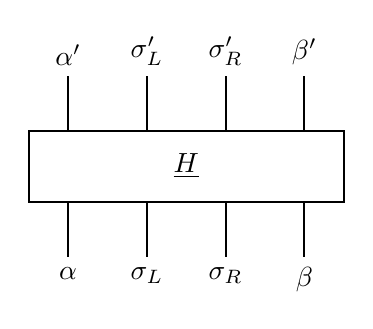
\begin{tikzpicture}[thick]
  \draw (0,0) rectangle (4,0.9);
  \node at (2,0.45) {$\underline{H}$};
  \foreach \x/\lab in {0.5/{\alpha'}, 1.5/{\sigma_L'}, 2.5/{\sigma_R'}, 3.5/{\beta'}}
    \draw (\x,0.9) -- (\x,1.6) node[above] {$\lab$};
  \foreach \x/\lab in {0.5/{\alpha}, 1.5/{\sigma_L}, 2.5/{\sigma_R}, 3.5/{\beta}}
    \draw (\x,0) -- (\x,-0.7) node[below] {$\lab$};
\end{tikzpicture}
\end{center}

denotes a matrix

\begin{equation}
\big(\underline{H}\big)_{\alpha\sigma_L\sigma_R\beta,\;\alpha'\sigma_L'\sigma_R'\beta'},
\end{equation}

the labels on the legs denote the basis. This notation specifically
chooses the up-legs as indexing the columns and the down-legs to index
the rows.

In the case of the remaining matrices

\begin{center}
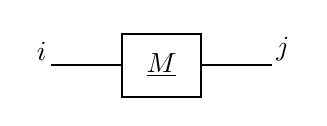
\begin{tikzpicture}[thick]
  \draw (0,0) rectangle (1,0.8);
  \node at (0.5,0.4) {$\underline{M}$};
  \draw (0,0.4) -- (-0.9,0.4) node[above left=-2pt] {$i$};
  \draw (1,0.4) -- (1.9,0.4) node[above right=-2pt] {$j$};
\end{tikzpicture}
\end{center}

represents $\big(\underline{M}\big)_{i,j}$, so the left legs index the
rows and the right legs index the columns.

In the case of multiple legs the order is to be interpreted as follows:

\begin{center}
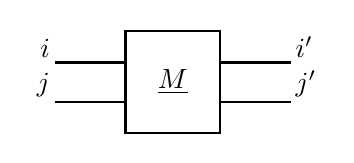
\begin{tikzpicture}[thick]
  \draw (0,0) rectangle (1.2,1.3);
  \node at (0.6,0.65) {$\underline{M}$};
  \draw (0,0.9) -- (-0.9,0.9) node[above left=-2pt] {$i$};
  \draw (0,0.4) -- (-0.9,0.4) node[above left=-2pt] {$j$};
  \draw (1.2,0.9) -- (2.1,0.9) node[above right=-2pt] {$i'$};
  \draw (1.2,0.4) -- (2.1,0.4) node[above right=-2pt] {$j'$};
\end{tikzpicture}
\end{center}

represents $\big(\underline{M}\big)_{ij,\;i'j'}$.

\paragraph{Algorithm in tensor notation.}

\begin{enumerate}
\item Compute the ground state
\begin{equation}
|\Psi_0\rangle = \sum_{\alpha\sigma_L\sigma_R\beta}\big(\vec\Psi_0\big)_{\alpha\sigma_L\sigma_R\beta}\;\big|\alpha\sigma_L\sigma_R\beta\big\rangle
\end{equation}
with energy $E_{0}^{i}$ of the Hamiltonian:

\begin{center}
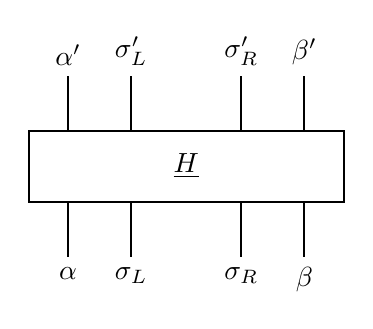
\begin{tikzpicture}[thick]
  \draw (0,0) rectangle (4,0.9);
  \node at (2,0.45) {$\underline{H}$};
  \foreach \x/\lab in {0.5/{\alpha'}, 1.3/{\sigma_L'}, 2.7/{\sigma_R'}, 3.5/{\beta'}}
    \draw (\x,0.9) -- (\x,1.6) node[above] {$\lab$};
  \foreach \x/\lab in {0.5/{\alpha}, 1.3/{\sigma_L}, 2.7/{\sigma_R}, 3.5/{\beta}}
    \draw (\x,0) -- (\x,-0.7) node[below] {$\lab$};
\end{tikzpicture}
\end{center}

compute energy density:

\begin{equation}
    e^{i} = (E_{0}^{i}-E_{0}^{i-1})/2
\end{equation}

iterate until $e^{i}$ converges.

\item Reshape to
\begin{equation}
\big(\underline{\Psi}_0\big)_{\alpha\sigma_L,\;\sigma_R\beta} = \big(\vec\Psi_0\big)_{\alpha\sigma_L\sigma_R\beta}
\end{equation}

\item Compute the SVD of $\underline{\Psi}_0 = \underline{U}\,\underline{S}\,\underline{V}^{\dagger}$.

\item Only keep the $\chi_{\max}$ largest singular values:
\begin{equation}
\underline{\Psi}_0^{(\mathrm{red})} = \underline{U}^{(\mathrm{red})}\,\underline{S}^{(\mathrm{red})}\,\big(\underline{V}^{(\mathrm{red})}\big)^{\dagger}
\end{equation}

\item Find the Hamiltonian in the new basis with $\underline{U}^{(\mathrm{red})}$ and $\underline{V}^{(\mathrm{red})}$ (the (red) label is dropped in favor of greater readability):

\begin{center}
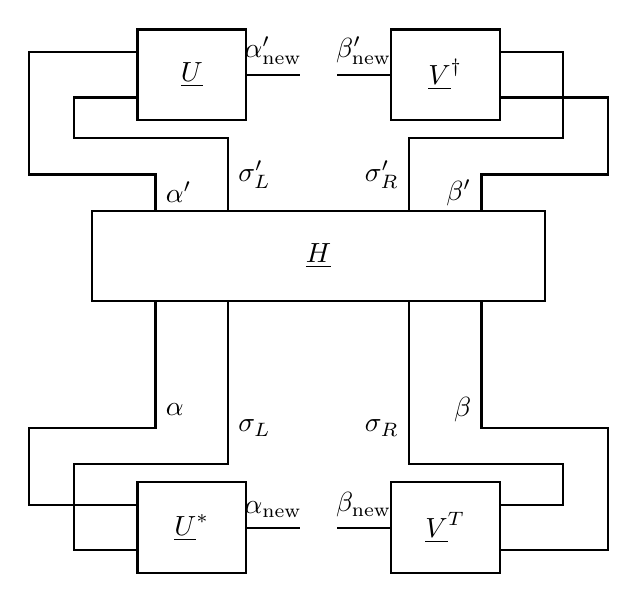
\begin{tikzpicture}[thick, scale=1.15]
  % Hamiltonian
  \draw (0,0) rectangle (5,1);
  \node at (2.5,0.5) {$\underline{H}$};
  % upper tensors
  \draw (0.5,2.0) rectangle (1.7,3.0);
  \node at (1.1,2.5) {$\underline{U}$};
  \draw (3.3,2.0) rectangle (4.5,3.0);
  \node at (3.9,2.5) {$\underline{V}^{\dagger}$};
  % lower tensors
  \draw (0.5,-3.0) rectangle (1.7,-2.0);
  \node at (1.1,-2.5) {$\underline{U}^{*}$};
  \draw (3.3,-3.0) rectangle (4.5,-2.0);
  \node at (3.9,-2.5) {$\underline{V}^{T}$};
  % upper left: alpha' into the upper slot, sigma_L' into the lower slot
  \draw (0.7,1) -- (0.7,1.4) -- (-0.7,1.4) -- (-0.7,2.75) -- (0.5,2.75);
  \node[right] at (0.7,1.2) {$\alpha'$};
  \draw (1.5,1) -- (1.5,1.8) -- (-0.2,1.8) -- (-0.2,2.25) -- (0.5,2.25);
  \node[right] at (1.5,1.4) {$\sigma_L'$};
  % upper right: sigma_R' crosses beta' to reach the upper slot
  \draw (3.5,1) -- (3.5,1.8) -- (5.2,1.8) -- (5.2,2.75) -- (4.5,2.75);
  \node[left] at (3.5,1.4) {$\sigma_R'$};
  \draw (4.3,1) -- (4.3,1.4) -- (5.7,1.4) -- (5.7,2.25) -- (4.5,2.25);
  \node[left] at (4.3,1.2) {$\beta'$};
  % new indices
  \draw (1.7,2.5) -- (2.3,2.5);
  \node[above] at (2.0,2.5) {$\alpha_{\mathrm{new}}'$};
  \draw (3.3,2.5) -- (2.7,2.5);
  \node[above] at (3.0,2.5) {$\beta_{\mathrm{new}}'$};
  % lower left: alpha crosses sigma_L to reach the upper slot
  \draw (0.7,0) -- (0.7,-1.4) -- (-0.7,-1.4) -- (-0.7,-2.25) -- (0.5,-2.25);
  \node[right] at (0.7,-1.2) {$\alpha$};
  \draw (1.5,0) -- (1.5,-1.8) -- (-0.2,-1.8) -- (-0.2,-2.75) -- (0.5,-2.75);
  \node[right] at (1.5,-1.4) {$\sigma_L$};
  % lower right: sigma_R already above beta, no crossing
  \draw (3.5,0) -- (3.5,-1.8) -- (5.2,-1.8) -- (5.2,-2.25) -- (4.5,-2.25);
  \node[left] at (3.5,-1.4) {$\sigma_R$};
  \draw (4.3,0) -- (4.3,-1.4) -- (5.7,-1.4) -- (5.7,-2.75) -- (4.5,-2.75);
  \node[left] at (4.3,-1.2) {$\beta$};
  \draw (1.7,-2.5) -- (2.3,-2.5);
  \node[above] at (2.0,-2.5) {$\alpha_{\mathrm{new}}$};
  \draw (3.3,-2.5) -- (2.7,-2.5);
  \node[above] at (3.0,-2.5) {$\beta_{\mathrm{new}}$};
\end{tikzpicture}
\end{center}

\end{enumerate}

\textbf{Note:} The $\underline{V}^{*}$ in the projective basis change formula \eqref{eq:projective-basis-trafo-right}
becomes $\underline{V}^{\dagger}$ in the tensor notation, since the legs that leave the box on 
the right side correspond to the columns.

\paragraph{Example: Hamiltonian of the first two iterations.}
The $(\mathrm{red})$ label will be dropped, so $\underline{U}^{(1)}$ and
$\underline{U}^{(2)}$, etc., do refer to the reduced versions. The
matrix underbars will also be neglected, so
$U^{(1)} = \underline{U}^{(1)(\mathrm{red})}$.

Start with original Hamiltonian acting on two sites:

\begin{center}
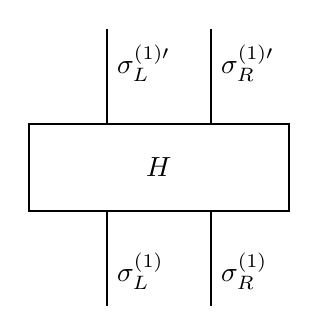
\begin{tikzpicture}[thick, scale=1.1]
  % Hamiltonian
  \draw (0,0) rectangle (3,1);
  \node at (1.5,0.5) {$H$};
  % upper legs
  \draw (0.9,1) -- (0.9,2.1);
  \node[right] at (0.9,1.7) {$\sigma_L^{(1)\prime}$};
  \draw (2.1,1) -- (2.1,2.1);
  \node[right] at (2.1,1.7) {$\sigma_R^{(1)\prime}$};
  % lower legs
  \draw (0.9,0) -- (0.9,-1.1);
  \node[right] at (0.9,-0.7) {$\sigma_L^{(1)}$};
  \draw (2.1,0) -- (2.1,-1.1);
  \node[right] at (2.1,-0.7) {$\sigma_R^{(1)}$};
\end{tikzpicture}
\end{center}

apply the projective basis change:

\begin{center}
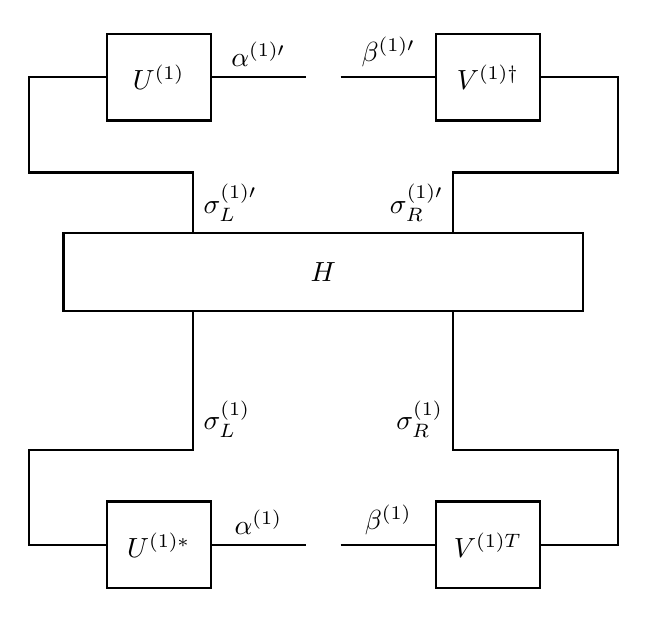
\begin{tikzpicture}[thick, scale=1.1]
  % Hamiltonian
  \draw (0,0) rectangle (6,0.9);
  \node at (3,0.45) {$H$};
  % upper boxes
  \draw (0.5,2.2) rectangle (1.7,3.2);
  \node at (1.1,2.7) {$U^{(1)}$};
  \draw (4.3,2.2) rectangle (5.5,3.2);
  \node at (4.9,2.7) {$V^{(1)\dagger}$};
  % lower boxes
  \draw (0.5,-3.2) rectangle (1.7,-2.2);
  \node at (1.1,-2.7) {$U^{(1)*}$};
  \draw (4.3,-3.2) rectangle (5.5,-2.2);
  \node at (4.9,-2.7) {$V^{(1)T}$};
  % upper: sigma_L^(2)' wraps around left into U
  \draw (1.5,0.9) -- (1.5,1.6) -- (-0.4,1.6) -- (-0.4,2.7) -- (0.5,2.7);
  \node[right] at (1.5,1.25) {$\sigma_L^{(1)\prime}$};
  % alpha^(1)' free leg out of U
  \draw (1.7,2.7) -- (2.8,2.7);
  \node[above] at (2.25,2.7) {$\alpha^{(1)\prime}$};
  % beta^(1)' free leg into V^dagger
  \draw (3.2,2.7) -- (4.3,2.7);
  \node[above] at (3.75,2.7) {$\beta^{(1)\prime}$};
  % V^dagger right leg wraps back into H
  \draw (5.5,2.7) -- (6.4,2.7) -- (6.4,1.6) -- (4.5,1.6) -- (4.5,0.9);
  \node[left] at (4.5,1.25) {$\sigma_R^{(1)\prime}$};
  % lower mirror
  \draw (1.5,0) -- (1.5,-1.6) -- (-0.4,-1.6) -- (-0.4,-2.7) -- (0.5,-2.7);
  \node[right] at (1.5,-1.25) {$\sigma_L^{(1)}$};
  \draw (1.7,-2.7) -- (2.8,-2.7);
  \node[above] at (2.25,-2.7) {$\alpha^{(1)}$};
  \draw (3.2,-2.7) -- (4.3,-2.7);
  \node[above] at (3.75,-2.7) {$\beta^{(1)}$};
  \draw (5.5,-2.7) -- (6.4,-2.7) -- (6.4,-1.6) -- (4.5,-1.6) -- (4.5,0);
  \node[left] at (4.5,-1.25) {$\sigma_R^{(1)}$};
\end{tikzpicture}
\end{center}

insert the next two sites:

\begin{center}
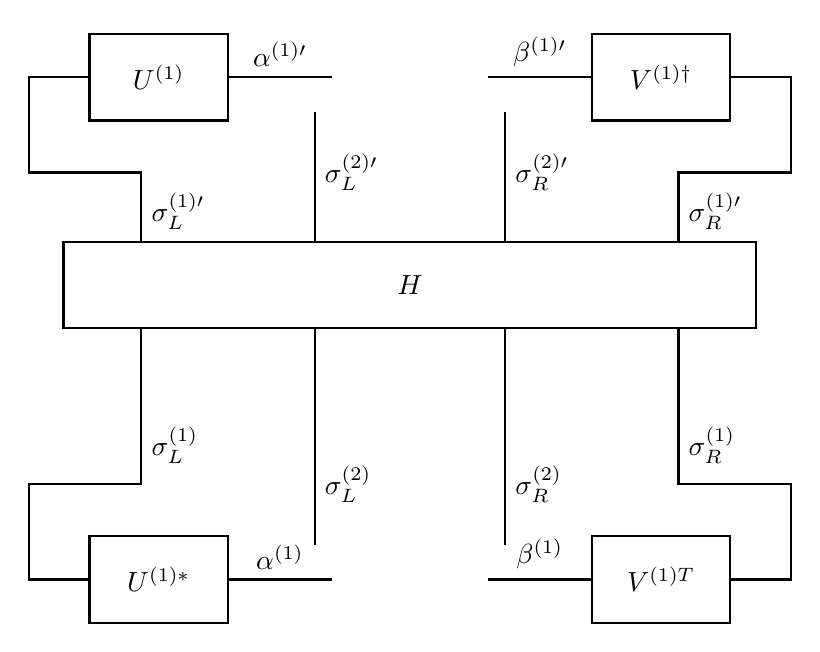
\begin{tikzpicture}[thick, scale=1.1]
  % Hamiltonian: four legs up, four legs down
  \draw (0,0) rectangle (8,1);
  \node at (4,0.5) {$H$};
  % upper boxes
  \draw (0.3,2.4) rectangle (1.9,3.4);
  \node at (1.1,2.9) {$U^{(1)}$};
  \draw (6.1,2.4) rectangle (7.7,3.4);
  \node at (6.9,2.9) {$V^{(1)\dagger}$};
  % lower boxes
  \draw (0.3,-3.4) rectangle (1.9,-2.4);
  \node at (1.1,-2.9) {$U^{(1)*}$};
  \draw (6.1,-3.4) rectangle (7.7,-2.4);
  \node at (6.9,-2.9) {$V^{(1)T}$};
  % --- upper legs of H ---
  % leg 1: sigma_L^(1)' -> wraps left into U
  \draw (0.9,1) -- (0.9,1.8) -- (-0.4,1.8) -- (-0.4,2.9) -- (0.3,2.9);
  \node[right] at (0.9,1.35) {$\sigma_L^{(1)\prime}$};
  % leg 2: sigma_L^(2)' free
  \draw (2.9,1) -- (2.9,2.5);
  \node[right] at (2.9,1.8) {$\sigma_L^{(2)\prime}$};
  % leg 3: sigma_R^(2)' free
  \draw (5.1,1) -- (5.1,2.5);
  \node[right] at (5.1,1.8) {$\sigma_R^{(2)\prime}$};
  % leg 4: sigma_R^(1)' -> wraps right into V
  \draw (7.1,1) -- (7.1,1.8) -- (8.4,1.8) -- (8.4,2.9) -- (7.7,2.9);
  \node[right] at (7.1,1.35) {$\sigma_R^{(1)\prime}$};
  % free indices from U and V (upper)
  \draw (1.9,2.9) -- (3.1,2.9);
  \node[above] at (2.5,2.9) {$\alpha^{(1)\prime}$};
  \draw (4.9,2.9) -- (6.1,2.9);
  \node[above] at (5.5,2.9) {$\beta^{(1)\prime}$};
  % --- lower legs of H (mirror) ---
  \draw (0.9,0) -- (0.9,-1.8) -- (-0.4,-1.8) -- (-0.4,-2.9) -- (0.3,-2.9);
  \node[right] at (0.9,-1.35) {$\sigma_L^{(1)}$};
  \draw (2.9,0) -- (2.9,-2.5);
  \node[right] at (2.9,-1.8) {$\sigma_L^{(2)}$};
  \draw (5.1,0) -- (5.1,-2.5);
  \node[right] at (5.1,-1.8) {$\sigma_R^{(2)}$};
  \draw (7.1,0) -- (7.1,-1.8) -- (8.4,-1.8) -- (8.4,-2.9) -- (7.7,-2.9);
  \node[right] at (7.1,-1.35) {$\sigma_R^{(1)}$};
  \draw (1.9,-2.9) -- (3.1,-2.9);
  \node[above] at (2.5,-2.9) {$\alpha^{(1)}$};
  \draw (4.9,-2.9) -- (6.1,-2.9);
  \node[above] at (5.5,-2.9) {$\beta^{(1)}$};
\end{tikzpicture}
\end{center}

apply next projective bassis change:

\begin{center}
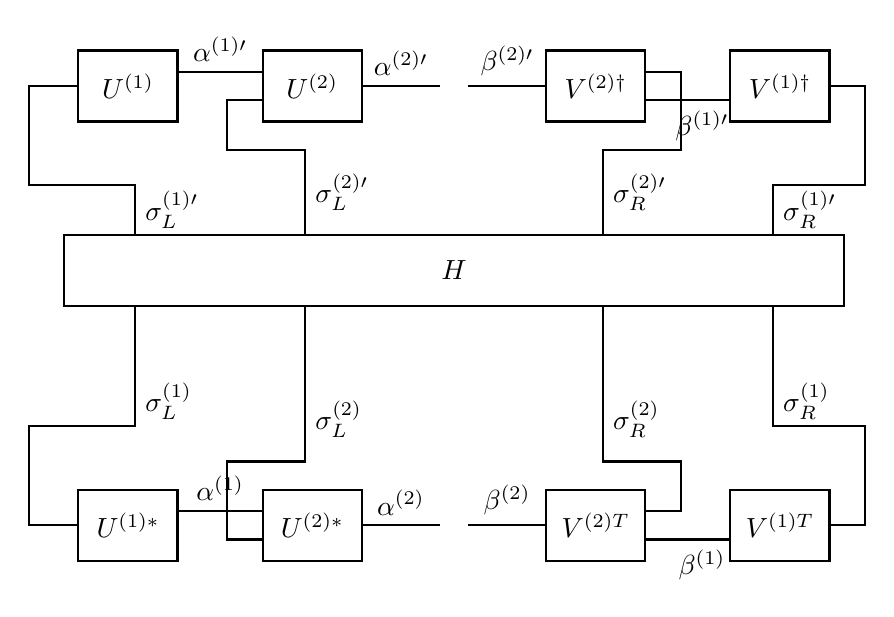
\begin{tikzpicture}[thick, scale=0.9]
  % Hamiltonian
  \draw (0,0) rectangle (11,1);
  \node at (5.5,0.5) {$H$};
  % upper boxes
  \draw (0.2,2.6) rectangle (1.6,3.6);  \node at (0.9,3.1) {$U^{(1)}$};
  \draw (2.8,2.6) rectangle (4.2,3.6);  \node at (3.5,3.1) {$U^{(2)}$};
  \draw (6.8,2.6) rectangle (8.2,3.6);  \node at (7.5,3.1) {$V^{(2)\dagger}$};
  \draw (9.4,2.6) rectangle (10.8,3.6); \node at (10.1,3.1) {$V^{(1)\dagger}$};
  % lower boxes
  \draw (0.2,-3.6) rectangle (1.6,-2.6);  \node at (0.9,-3.1) {$U^{(1)*}$};
  \draw (2.8,-3.6) rectangle (4.2,-2.6);  \node at (3.5,-3.1) {$U^{(2)*}$};
  \draw (6.8,-3.6) rectangle (8.2,-2.6);  \node at (7.5,-3.1) {$V^{(2)T}$};
  \draw (9.4,-3.6) rectangle (10.8,-2.6); \node at (10.1,-3.1) {$V^{(1)T}$};
  % --- upper wiring ---
  \draw (1.0,1) -- (1.0,1.7) -- (-0.5,1.7) -- (-0.5,3.1) -- (0.2,3.1);
  \node[right] at (1.0,1.35) {$\sigma_L^{(1)\prime}$};
  \draw (1.6,3.3) -- (2.8,3.3);
  \node[above] at (2.2,3.3) {$\alpha^{(1)\prime}$};
  \draw (3.4,1) -- (3.4,2.2) -- (2.3,2.2) -- (2.3,2.9) -- (2.8,2.9);
  \node[right] at (3.4,1.6) {$\sigma_L^{(2)\prime}$};
  \draw (4.2,3.1) -- (5.3,3.1);
  \node[above] at (4.75,3.1) {$\alpha^{(2)\prime}$};
  \draw (5.7,3.1) -- (6.8,3.1);
  \node[above] at (6.25,3.1) {$\beta^{(2)\prime}$};
  % sigma_R^(2)' crosses the beta^(1)' line
  \draw (7.6,1) -- (7.6,2.2) -- (8.7,2.2) -- (8.7,3.3) -- (8.2,3.3);
  \node[right] at (7.6,1.6) {$\sigma_R^{(2)\prime}$};
  \draw (8.2,2.9) -- (9.4,2.9);
  \node[below] at (9.0,2.9) {$\beta^{(1)\prime}$};
  \draw (10.8,3.1) -- (11.3,3.1) -- (11.3,1.7) -- (10.0,1.7) -- (10.0,1);
  \node[right] at (10.0,1.35) {$\sigma_R^{(1)\prime}$};
  % --- lower wiring ---
  \draw (1.0,0) -- (1.0,-1.7) -- (-0.5,-1.7) -- (-0.5,-3.1) -- (0.2,-3.1);
  \node[right] at (1.0,-1.35) {$\sigma_L^{(1)}$};
  \draw (1.6,-2.9) -- (2.8,-2.9);
  \node[above] at (2.2,-2.9) {$\alpha^{(1)}$};
  % sigma_L^(2) crosses the alpha^(1) line
  \draw (3.4,0) -- (3.4,-2.2) -- (2.3,-2.2) -- (2.3,-3.3) -- (2.8,-3.3);
  \node[right] at (3.4,-1.6) {$\sigma_L^{(2)}$};
  \draw (4.2,-3.1) -- (5.3,-3.1);
  \node[above] at (4.75,-3.1) {$\alpha^{(2)}$};
  \draw (5.7,-3.1) -- (6.8,-3.1);
  \node[above] at (6.25,-3.1) {$\beta^{(2)}$};
  \draw (7.6,0) -- (7.6,-2.2) -- (8.7,-2.2) -- (8.7,-2.9) -- (8.2,-2.9);
  \node[right] at (7.6,-1.6) {$\sigma_R^{(2)}$};
  \draw (8.2,-3.3) -- (9.4,-3.3);
  \node[below] at (9.0,-3.3) {$\beta^{(1)}$};
  \draw (10.8,-3.1) -- (11.3,-3.1) -- (11.3,-1.7) -- (10.0,-1.7) -- (10.0,0);
  \node[right] at (10.0,-1.35) {$\sigma_R^{(1)}$};
\end{tikzpicture}
\end{center}

\subsection{MPS Implementation}

The tensor notation is the notation developed by Jan von Delft and demonstrated in his lecture \cite{tensornetworks}.
The derivations also followly ate least loosely the derivations in the lecture.

DMRG is a Tensor Network Method for determining the ground state of a Hamiltonian. 
The method minimizes the energy $\langle \psi | \hat{H} | \psi \rangle$ under the constraint that the state remains normalized $\langle \psi | \psi \rangle = 1$. 
A straightforward approach is using a Lagrange multiplier and minimizing the cost function:
\begin{equation}
    \langle \psi | \hat{H} | \psi \rangle - \lambda\big( \langle \psi | \psi \rangle - 1 \big) \label{eq:DMRG-cost}
\end{equation}

We want to minimize the above expression with respect to the tensors $[T_i]_{k_{i-1},\sigma_i,k_i}$ where
\begin{equation*}
    [\psi]_{\sigma_1 \dots \sigma_L} = \sum_{k_2} \dots \sum_{k_{L}} [T_1]_{k_1 \sigma_1 k_2} \dots [T_L]_{k_L \sigma_L k_{L+1}}
\end{equation*}
$k_1$ and $k_{L+1}$ are dummy indices and
\begin{equation*}
    |\psi\rangle = \sum_{\sigma_1} \dots \sum_{\sigma_L} [\psi]_{\sigma_1 \dots \sigma_L}\, |\sigma_1\rangle \otimes \dots \otimes |\sigma_L\rangle
\end{equation*}
with Hamiltonian

\begin{equation*}
\hat H = \sum_{\{\sigma\},\{\sigma'\}}
   [H]_{\sigma_1\dots\sigma_L\,\sigma_1'\dots\sigma_L'}\;
   |\sigma_1\dots\sigma_L\rangle\langle\sigma_1'\dots\sigma_L'|.
\end{equation*}

where the coefficents are given by:

\begin{equation*}
[H]_{\sigma_1\dots\sigma_L\,\sigma_1'\dots\sigma_L'} = \sum_{k_2}\cdots\sum_{k_L}
   [h_1]_{k_1\,\sigma_1\sigma_1'\,k_2}\cdots
   [h_L]_{k_L\,\sigma_L\sigma_L'\,k_{L+1}} \\[4pt]
\end{equation*}

Although the symbol $\sigma$ is commonly associated with spin degrees of freedom, her it denotes a general local physical index. 
For example, $\sigma_j$ may represent a site occupation number and is not necessarily binary. Its range is determined by the
dimension of the local physical Hilbert space.

In tensor notation, equation \eqref{eq:DMRG-cost} takes the form:

\begin{figure}[htbp]
  \centering
  \includegraphics[width=\linewidth]{figures/dmrg_cost.png}   % no extension needed
  \caption{DMRG cost function $\langle\psi|\hat H|\psi\rangle - \lambda(\langle\psi|\psi\rangle - 1)$
           in tensor-network form. The MPS is in site-canonical form with respect to the site $i$.}
  \label{fig:dmrg_cost}
\end{figure}

Taking the derivative by $\frac{\partial}{\partial A_i^{\dagger}}$ we find \ref{fig:dmrg_eigen_problem}, which is just a standard eigenvalue problem in graphical notation for the effective Hamiltonian \ref{fig:dmrg_effective_hamiltonian}.


\begin{figure}[htbp]
  \centering
  \includegraphics[width=\linewidth]{figures/dmrg_eigenproblem.png}   % no extension needed
  \caption{DMRG eigenvalue problem in graphical notation.}
  \label{fig:dmrg_eigen_problem}
\end{figure}

\begin{figure}[htbp]
  \centering
  \includegraphics[width=\linewidth]{figures/dmrg_effective_hamiltonian.png}   % no extension needed
  \caption{DMRG effective Hamiltonian in graphical notation.}
  \label{fig:dmrg_effective_hamiltonian}
\end{figure}

The derivative by $\lambda$ just leads to the auxiliary condition that the eigenvector 
of the eigenvalue problem has to be normalized.
The updated tensor $T_i$ is choosen as the (normalized) ground state of the effective Hamiltonian.
A shift of the active site is performed by applying a QR-decomposition followed by a tensor contraction. 
The only heuristic choices in this algorithm are the ranks of the original state, which can not be increased and 
the choice of the ground state of the effective Hamiltonian as the updated tensor $T_i$ in the ground state of the entire Hamitonian.

The MPO representation of the Hamiltonian can alternatively be expressed as a sum of, easier to interpret, $n$-tensor operators. 
As an example, consider the non-interacting Hubbard Hamiltonian. The hopping terms correspond to identical two-site operators acting
on neighbouring sites, while the chemical potential terms are represented by identical one-site operators.
In $k$-space we would only find one-site operators, which would differ for every site.
Figure \ref{fig:effective-hamiltonian-one-two-site} demonstrates the effective Hamiltonian in that case.

\begin{figure}[htbp]
  \centering
  \includegraphics[width=\linewidth]{figures/effective_hamiltonian_one_two_site.png}   % no extension needed
  \caption{Effective Hamiltonian with translation invariant one- and two-site operators.}
  \label{fig:effective-hamiltonian-one-two-site}
\end{figure}

To find excited states or treat ground state degeneracy with DMRG, one must add another
Langrange multiplier term to the cost function \eqref{eq:DMRG-cost}: 

\begin{equation*}
    \langle\psi|\hat H|\psi\rangle
    - \lambda_1\big(\langle\psi|\psi\rangle - 1\big)
    - \lambda_2\,\langle\psi|\phi\rangle - \bar{\lambda_2}\,\langle\phi|\psi\rangle
\end{equation*}

where $|\phi\rangle$ is the state and $|\psi\rangle$ should be orthogonal to, for example, the result from the previous DMRG calculation.
Again by differentiating with respect to $T_i$ we find the effective vector $|\phi_{eff}\rangle$ sketched in figure \ref{fig:effective-vector}.
With this vector one can build the projector:

\begin{equation*}
    \hat P = \mathbb{1} - |\phi_{\text{eff}}\rangle\langle\phi_{\text{eff}}|
\end{equation*}

and solve the eigenproblem of the effective Hamiltonian (figure \ref{fig:dmrg_eigen_problem}) in the projected space:

\begin{equation*}
    \hat P\,\hat H_{\text{eff}}\,\hat P\,|\psi_i\rangle = \lambda\,\hat P\,|\psi_i\rangle
\end{equation*}

\begin{figure}[htbp]
  \centering
  \includegraphics[width=\linewidth]{figures/DMRG_effective_vector.png}   % no extension needed
  \caption{Effective Vector $|\phi_{eff}\rangle$. Where the double triangles denote state $|\phi\rangle$}
  \label{fig:effective-vector}
\end{figure}

Generalizing single-site DMRG from an MPS structure to a general TTN structure does not change the 
essence of the algorithm. The optimization problem still reduces to a one-site effective eigenproblem.
However, the traversing pattern needs to be changed to a depth first pattern, 
where we only start updating the nodes once we reach the first leaf.
As we continue with the depth first traversion pattern, 
every node that is traversed and was not yet updated, will
be updated. Traversing here means not just moving from tensor to tensor, 
but moving the canonical site i. Moving the canonical
site i is achieved via QR-decompositions followed by contractions, as in the MPS case. 
The iteration ends if the canonical site is at the 
starting point and there are no neighbouring nodes/tensors that have not been updated.




\section{TDVP}
The time-dependent variational principle (TDVP) is a tensor network method, like DMRG,
but used to time-evolve a TTN or MPS state. The algorithm is based on the observation
that the time derivative of a tensor network lies in the tangent space of that network,
i.e.\ the space spanned by all tensor networks that differ from the original by a single
tensor. Thus, if the original network consists of $n$ tensors, its tangent space is
spanned by $n$ states, one for each tensor. Crucially, $\hat H |\psi\rangle$ does not
necessarily lie in this space, and the idea of the TDVP algorithm is to force
$\hat H |\psi\rangle$ into the tangent space. Figure~\ref{fig:tangent-space-projector}
shows the tangent space projector.

Let us briefly argue that the tangent space projector indeed imposes the structure of
the derivative onto $\hat H |\psi\rangle$. I follow the approach of Jan von Delft, but
ignore the notion of kept and discarded spaces in the derivation. I will not show that
the tangent space projector is in fact a projector: this is considerably easier with the
kept and discarded spaces, and I have nothing to add to von Delft's derivation \cite{tensornetworks}.
\begin{figure}[htbp]
\centering
\includegraphics[width=\linewidth]{figures/tangent-space-projector.png}
\caption{Tangent space projector.}
\label{fig:tangent-space-projector}
\end{figure}
We have the QR relationship shown in Figure~\ref{fig:QR-decomp} between the site tensors
$T_i$, the left isometries $A_i$, and the matrices $R_i$. Differentiating the QR
decomposition yields the relation in Figure~\ref{fig:left-iso-derivative} for the
derivative of the left isometry $A_i$. Using contractions and QR decompositions, one can
move the matrix $R_i$ and thereby place the canonical site in the desired position. Note
that the left-hand side of the equation is then completed by left and right isometries
alone.
\begin{figure}[htbp]
\centering
\includegraphics[width=\linewidth]{figures/QR-decomp.png}
\caption{QR decomposition in graphical notation.}
\label{fig:QR-decomp}
\end{figure}
\begin{figure}[htbp]
\centering
\includegraphics[width=\linewidth]{figures/left-isometry-derivative.png}
\caption{Derivative of the left isometry.}
\label{fig:left-iso-derivative}
\end{figure}
With this relation in hand, we can compute the time derivative of the entire MPS. We take
the MPS to be in site-canonical form, with the canonical site in the rightmost position
$L$. Figure~\ref{fig:derivative-MPS} shows the resulting derivative. Comparing its
structure to the tangent space projector in Figure~\ref{fig:tangent-space-projector}, one
immediately sees that the two match exactly. We therefore obtain a differential equation
for each tensor $T_i$ and each matrix $R_i$.
\begin{figure}[htbp]
\centering
\includegraphics[width=\linewidth]{figures/derivative-MPS.png}
\caption{Derivative of the entire MPS.}
\label{fig:derivative-MPS}
\end{figure}
We can now use the time-evolution operators provided by these differential equations to
evolve the MPS. To see how this works, again assume the MPS is in site-canonical form
with the canonical site at $L$, and start at site $1$. We want to find $A_1(t_0+t)$:
applying the time-evolution operator for $T_1$ gives
$T_1(t_0+t) = A_1(t_0+t)\,R_1(t_0+t)$, from which we read off $A_1(t_0+t)$. To find
$A_2(t_0+t)$, however, we must time-evolve $T_2(t_0) = R_1(t_0)\,A_2(t_0)$, which requires
evolving the bond matrix $R_1$ backward in time. The procedure continues in the same way
until we reach the last tensor $T_L(t_0)$.

\textbf{Note:} The isometries have to be understood as the site-canonical isometries,
even in the bond representation. As a consequence,
the bond matrices are not necessarily diagonal. Moreover, all references to a QR decomposition imply the reduced (thin) QR decomposition.

\section{Application: Fast Fourier Transform (FFT)}

By comparing the physics convention (left) with the computer-science
convention (\texttt{scipy}) on the right in \eqref{eq:fft-physics-conv}:
\begin{equation}\label{eq:fft-physics-conv}
  \exp(i\,\omega_k t_n) \;\overset{!}{=}\; \exp\!\Big(i\,2\pi k\,\tfrac{n}{N}\Big)
\end{equation}

one obtains
\begin{equation*}\label{eq:fft-omega-t}
  \omega_k := \frac{2\pi k}{t_{\text{end}} - t_{\text{start}}},
  \qquad
  t_n := \Delta t \cdot n .
\end{equation*}

\subsection{Fast Fourier Transform of a Delta Function}

We assume the same realization of the delta function that we have been
assuming throughout, only we do not take the limit $\eta \to 0$.
This is characterized by a transition from a delta function $\delta(x)$ to a Lorentzian $L(x)$:
\begin{equation*}\label{eq:delta-lorentzian}
  L(\omega_k - \varepsilon)
  = \frac{1}{\pi}\,\frac{\eta}{(\omega_k - \varepsilon)^2 + \eta^2},
\end{equation*}
and we want to calculate the correct normalization constant $C$ of the
Fourier transform:
\begin{equation*}\label{eq:fft-delta-sum}
  C\, \sum_{k=1}^{N}
     \exp\!\Big(i\,2\pi k\,\tfrac{n}{N}\Big)\,
     L(\omega_k - \varepsilon)
\end{equation*}

\paragraph{Case: $\Delta\omega \gg \eta$.}
In this scenario one will only ``hit'' the delta function if
$\varepsilon \in \Omega$ with $\Omega = \{\,\omega_k \mid k \in [1, N]\,\}$.
The value of the delta function at this position is given by
\begin{equation*}\label{eq:delta-peak}
  L(\varepsilon - \varepsilon) = \frac{1}{\pi\eta}.
\end{equation*}
Therefore, one has to choose
\begin{equation*}\label{eq:fft-C}
  C = \pi\eta .
\end{equation*}

\paragraph{Case: $\Delta\omega \approx \eta$.}
This case is considered as academic study to create a smoother transition to the next case. In practice, one
will either use the previous case, if possible, or approximate the normalization constant by the one in the integration limit.
The Fourier transform now requires the normalization factor:
\begin{equation*}\label{eq:fft-C-intermediate}
  C = \frac{\pi}{\displaystyle\sum_{k}\frac{\eta}{(\omega_k - \varepsilon)^2 + \eta^2}} .
\end{equation*}


\paragraph{Case: $\Delta\omega \ll \eta$.}
In this limit we assume that
\begin{equation*}\label{eq:fft-sum-to-integral}
  \Delta\omega \sum_{k}\frac{\eta}{(\omega_k - \varepsilon)^2 + \eta^2}
  \;\approx\;
  \int d\omega\,\frac{\eta}{(\omega - \varepsilon)^2 + \eta^2}
  \;=\; \pi .
\end{equation*}
And thus we find
\begin{equation*}\label{eq:fft-C-final}
  C = \Delta\omega .
\end{equation*}

This is the most reliable case, and therefore we want
$\Delta\omega \ll \eta$. For small $\eta$, we must compute the evolution over a long period of time. 
In the case of imaginary time evolution a small $\eta$ also requires a long time 
evolution, to ensure sufficient decay.
